\section{Impegno orario}

Il tredicesimo gruppo composto da 7 studenti si impegna in toto a contribuire per ore \textbf{95} pro capite allo svolgimento del progetto didattico.

Suddette ore verranno suddivise come segue, tenendo conto dei ruoli definiti.

Viene inoltre applicato un \textbf{10\%} di coefficente di rendimento nel conteggio di ore reali rispetto alle ore produttive.

\begin{center}
    \begin{tabularx}{10cm}{X |l|l}          
        \textbf{Ruolo} & \textbf{Costo orario} & \textbf{Ore per ruolo}\\
        \hline

        Responsabile & §30 & 63\\
        Amministratore & §20 & 69\\
        Analista & §25 & 159\\
        Progettista & §25 & 152\\
        Programmatore & §15 & 152\\
        Verificatore & §15 & 97\\
        \hline
        \textbf{Totale} & §14197,75 & ore 692
    \end{tabularx}
\end{center}

La distribuzione per ruolo è quindi come segue.

\begin{center}
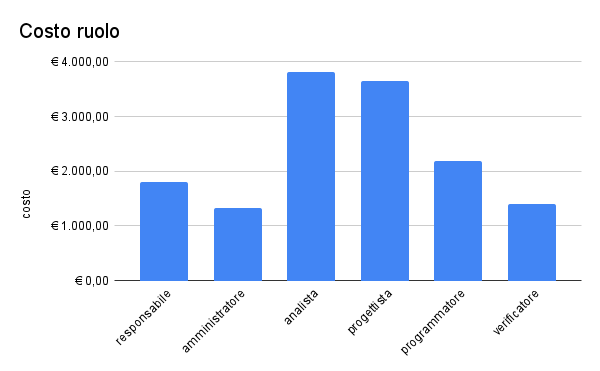
\includegraphics[width=0.8\textwidth]{immagini/Costo ruolo.png}
\end{center}

Ogni ruolo avrà inoltre rotazione costante e sistematica ma le ore preventivate per ogni studente si attestano a questi valori:

\begin{center}
    \begin{tabularx}{10cm}{X |l|l}          
        \textbf{Ruolo} & \textbf{Costo orario} & \textbf{Ore per ruolo}\\
        \hline

        Responsabile & §30 & 63\\
        Amministratore & §20 & 69\\
        Analista & §25 & 159\\
        Progettista & §25 & 152\\
        Programmatore & §15 & 152\\
        Verificatore & §15 & 97\\
        \hline
        \textbf{Totale} & §14197,75 & ore 692
    \end{tabularx}
\end{center}

\section{Considerazioni sui ruoli}
\section{Costi}

Il preventivo di realizzazione ammonta quindi a §14197,75 arrotondabili per eccesso a \textbf{§14200,00}

\section{Consegna}

La previsione di consegna chiavi in mano si attesta oggi al \textbf{06 marzo 2023}
